% vim: tw=0:wrap:linebreak
\documentclass[OPS,toc,lsstdraft]{lsstdoc}

\usepackage{comment}
\usepackage{datetime}
\usepackage{microtype}

\newcommand{\microarcsec}{$\mu$as\xspace}
\interfootnotelinepenalty=10000


\setcounter{secnumdepth}{3}

%%%%%%%%%%%%%%%%%%%%%
% Introduce mechanism to turn on and off various annotations (\XXX command,
% \begin{notes}, and anything else bracketed by \ifannotated ... \fi)
%
\newif\ifannotated
\annotatedtrue
\annotatedfalse	% uncomment this to hide all annotations (comments, notes, etc)

\ifannotated
	% leave things as-is
\else
	% hide all \XXX commands
	\renewcommand{\XXX}{}

	% hide all \begin{note}...\end{note} text
	\renewenvironment{note}[1][Note]
	{}
	{}
\fi
%%%%%%%%%%%%%%%%%%%%%

\title{LSST Processing of Gravitational Wave TOO Data in the Early Operations Era}
\author{
Eric~C.~Bellm
}

\input{meta}
\setDocRef{\lsstDocType-\lsstDocNum}
\setDocCurator{E.~Bellm}
\setDocDate{\vcsdate}
\setDocUpstreamVersion{\vcsrevision}
%\setDocUpstreamLocation{\url{https://github.com/lsst/LDM-723}}

%
%   Revision history
%
% OLDEST FIRST: VERSION, DATE, DESCRIPTION, OWNER NAME
\setDocChangeRecord{%
\addtohist{}{2019-12-16}{Initial draft version}{Eric Bellm}
}


\begin{document}


\setDocAbstract{%
Since the watershed discovery of an electromagnetic counterpart to the LIGO gravitational wave source GW170817, multi-messenger astrophysics has emerged as a major area of strategic focus for the NSF. 
LSST’s depth, survey speed, and data management systems will make it a key asset in the search for EM counterparts.  
Exploiting this capability in the first year of LSST operations (GW observing run O4) may require special actions, however.
We discuss potential approaches to data access, reference building, and special data processing.
}

\maketitle

\section{Scientific, Technical, and Programmatic Context}

The first binary neutron star merger detected in gravitational waves, GW170817, was detected at the end of observing run O2 \citep{2017PhRvL.119p1101A} along with coincident gamma-rays \citep{2017ApJ...848L..13A}.  
It was rapidly localized by many groups of electromagnetic observers \citep{2017ApJ...848L..12A}, enabling an unprecedented followup campaign.

Despite this initial success, intense followup of ten neutron-star-involved mergers to date in observing run O3 have not yielded a credible electromagnetic counterpart.
Absent a major shift in the discovery rate, it seems quite plausible that there will be no new counterpart identifications before O3 ends in April 2020.
Such a scenario would create substantial community and agency pressure on LSST, as LSST's major improvement in survey speed relative to current facilities is likely be necessary to make progress in this area \citep[e.g.,][]{2019arXiv191011246C}.

Indeed, LSST's depth and wide field of view provides great potential for discovery. 
LSST's strengths will become increasing important in later GW observing runs: 
as KAGRA and LIGO-India come online, GW spatial localizations will improve to $\sim$tens of square degrees, lessening the need for extremely wide-field instruments to tile major fractions of the sky.  
However, as the GW interferometers become more sensitive the GW sources detected will be farther away, making already-faint EM counterparts even fainter.

There will certainly be other EM followup programs active in the Southern Hemisphere, including the new BlackGEM array as well as community programs with DECam.
However, LSST is capable of making the definitive measurements, delivering high-impact early science along with another major NSF facility in an area of NSF strategic priority\footnote{``Windows on the Universe:'': \url{https://www.nsf.gov/news/special_reports/big_ideas/universe.jsp}}.

One challenge remains: the current timeline for future LIGO/Virgo/KAGRA observing runs (Figure \ref{fig:scenarios}) calls for observing run O4 to overlap with the LSST commissioning period and the first year of operations.
In this period prior to the first LSST data release (DR1), alert production will not be running at full volume or full fidelity.
Moreover, after O4 there will be a long, two-year period of downtime (until 2025+) for upgrades to the GW interferometers.  
Accordingly, there are high stakes for LSST to deliver EM counterparts in O4 despite the technical challenges it presents.

\begin{figure}
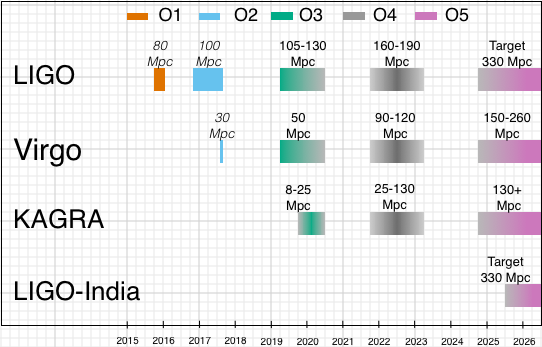
\includegraphics[width=\textwidth]{LVK_run_plan_190711.png}
\caption{Projected observing scenarios for LIGO, Virgo, KAGRA, and LIGO-India.  Retrieved 2019-12-11 from 
\url{https://www.ligo.org/scientists/GWEMalerts.php}.
	\label{fig:scenarios}}
\end{figure}

Critical LSST policy and survey strategy questions remain: who can decide to trigger a TOO, and with what observing sequences?  
We place these outside the scope of the present draft\footnote{We note that the realities of the LSST data in this timeframe suggest some constraints on observing strategy:  
Given the incompleteness of solar system catalogs, TOO observations should ensure two or more observations separated by an interval sufficient to reject main belt asteroids (minimally, 20 minutes, but larger separations would better capture the expected intranight temporal evolution of kilonovae).  
Since there will be minimal variability history, obtaining near-simultaneous exposures in at least two bands will enable searches for sources with extreme colors.  
These are consistent with the observing strategy proposed by \citet{2018arXiv181204051M}.} and assume that appropriately-developed TOO observations are being triggered.

This document asks what steps LSST can take to maximize the scientific value of any GW TOO observations undertaken in the early operations era (defined as the time before DR1, when Data-Release templates are available for all or most of the sky), with a particular emphasis on data processing, data products, and data availability.

LSST alerts are its real-time data product.  
In the commissioning and early operations era, 
templates will not available in many areas, and hence standard alert processing cannot be used to disseminate candidates.
If LSST templates exist in the area to be covered, standard LSST processing can proceed as normal (subject to the caveats described in \citeds{DMTN-065}).

Given the potentially high impact of the science, its visibility in the community, and importance to the NSF, we suggest that the operations project consider special handling of these TOO observations in the early operations era.  
(Similar considerations apply in commissioning.) 

The following analysis assumes that LSST TOO observations are relatively uncommon in this period (restricted to no more than 1 trigger/month, on average, perhaps) such that the staff impacts are tolerable.  
We assume that any triggers would be on relatively well-localized GW sources (a few LSST pointings), and so any additional data processing is well within operational compute margins.
These assumptions are in broad agreement with the followup proposal submitted by \citet{2018arXiv181204051M} in their response to the LSST call for cadence  white papers.

\section{Recommendations}

\subsection{Expedite data availability} \label{sec:data}

User access to raw and processed images is not required prior to 24 hours after the data are taken (\texttt{L1PublicT}; \texttt{LSR-REQ-0104} \citedsp{LSE-29}).  
Moreover, \texttt{LSR-REQ-0126} specifies that images and catalog products except for alerts are embargoed for a \textit{minimum} of \texttt{L1PublicTmin} = 6 hours before release to anyone \citedsp{LSE-29}.
Followup observations in the first 24 hours are among the most critical for constraining progenitor scenarios, so delays of this duration are unlikely to be viewed as acceptable by the community, particularly if they are not driven by technical limitations.

Current experience with DECam in particular suggests there will be a major community demand for user-generated processing, even starting with the raw imaging. 
Given the relatively few exposures expected, the compute and/or data-transfer needs for users are not onerous.
If the LSST imaging data is available in a timely manner, users may elect to perform processing beyond standard LSST processing, including differencing against templates from other surveys (e.g., DECaLS), cross-band image differencing to identify sources of extreme color, differencing of nightly stacks, alternative image differencing algorithms, etc.

Timely access to the images themselves is necessary to enable this user processing.
Given the high profile and priority of the science, we suggest that the LSST Operations Project attempt to secure an agency exemption from \texttt{LSR-REQ-0126} for TOO data specifically to enable rapid release ($<$1 hour) of the imaging data.
This may require developing alternative data release interfaces.

The question of data rights is also present here; we assume that by default access to imaging data would continue to be restricted to LSST Users \citedsp{LDO-13}.


\subsection{Conduct incremental template building} \label{sec:templates}

Standard alert processing provides the most rapid dissemination of candidate counterparts from TOO observations with the least operational burden, but it requires the existence of template images from prior LSST observations.

In \citeds{DMTN-107} the DM-SST suggests that incremental template generation in the first year of LSST operations provides the best balance of early template availability and artifact rejection.
In this scenario new templates are regularly generated throughout the year whenever sufficient imaging becomes available in sky areas and filters without templates.
Having preexisting templates will allow standard alert processing in GW TOO fields, easing the operational impacts of TOO observations.

Additionally, evidence of variability prior to the GW trigger provides one of the most effective ways to rule out unassociated sources in the GW localization region \citep[e.g.,][]{2019GCN.24223....1C, 2019GCN.26430....1S}.
At LSST depths there will be many unrelated events, and little recent prior imaging of sufficient depth from other surveys that can constrain the explosion date.
Already today at DECam followup depths the number of unrelated events is straining the ability of the worldwide community to obtain classification spectra \citep[e.g.,][]{2019ApJ...881L..16A}.

In the steady state survey, LSST's own history will provide substantial filtering: simply selecting \DIAObjects created after the the trigger will exclude most unrelated contaminants.
In early operations, however, this history will not be available, so not only distant supernovae but also variable stars and AGN will confound efforts to identify plausible GW counterparts.

For this reason it will be very helpful for LSST to have reliable standard image differencing processing---and hence history---as soon as is practical, providing further impetus for incremental template building.
While custom processing and association could be used to derive this history (\S \ref{sec:processing}) it would require substantial additional effort relative to LSST's standard processing.

If TOO observations are expected to be conducted in a subset of LSST's filters, any observations intended to maximize template coverage could prioritize obtaining images in those bands.

\subsection{Conduct bespoke image differencing on-project} \label{sec:processing}

Finally, we suggest that the operations team devote specific effort to custom processing and/or analysis of TOO observations.
This processing is most critical if the raw data cannot be made available to the community in a timely manner (\S \ref{sec:data}) and pre-existing templates are not available for the fields to be observed (\S \ref{sec:templates}).

In this scenario, the LSST Operations team would undertake a best-effort activity to produce \DIASources (and \DIAObjects, if possible) for the TOO observations.
The goal would not be to perform scientific analysis\footnote{though team members would not be precluded from doing so later} but to rapidly report reliable results to the community.
The team would use its judgment to undertake custom processing to enable the rapid identification of plausible counterparts.
This processing might include image-to-image differencing using prior LSST data, on-the-fly generation of new templates, or various flavors of forced photometry.

While it might be possible to generate functional alert packets to forward to community alert brokers, the team would also likely report results via other channels, in particular the GCN Circulars used by the broader EM/GW community.
As an extremely time-sensitive, alert-like product these results would be made world-public immediately.

LSST's TOOs will be highly visible, highly scrutinized observations, and so it will be valuable to have data processing performed by the highly-experience LSST operations team under the LSST imprimatur.
Successful execution of such processing will require a specialized team that will agree to be on-call in case of TOO triggers.
This team would consist primarily of LSST Operations personnel but could include key members of the Science Collaborations with relevant expertise (emphasizing again that the purpose of this activity is data processing, not science analysis).

It will be crucial to develop and rehearse procedures in advance to clarify authority, responsibility, and communications channels. 
In developing these procedures it would be useful to consult with the operations of other public facilities conducting EM/GW followup, such as \textit{Swift} and \textit{Fermi}.

During O4 the on-call team should be activated even in cases when templates exist for the TOO observations.
In this case custom processing might not be required, but the team would perform detailed QA of the alerts produced by the standard pipeline and report any problems with the automated analysis to the community via GCN.

%\clearpage
%\section{Acronyms}
%\addtocounter{table}{-1}
\begin{longtable}{p{0.145\textwidth}p{0.8\textwidth}}\hline
\textbf{Acronym} & \textbf{Description}  \\\hline

 &  \\\hline
AGN & active galactic nuclei \\\hline
DM & Data Management \\\hline
DM-SST & DM System Science Team \\\hline
DMTN & DM Technical Note \\\hline
DR1 & Data Release 1 \\\hline
GCN & GRB Coordinates Network \\\hline
GW & Gravitational Wave \\\hline
LDO & LSST Document Operations (Document Handle) \\\hline
LIGO & Laser Interferometer Gravitational-Wave Observatory \\\hline
LSE & LSST Systems Engineering (Document Handle) \\\hline
LSR & LSST System Requirements; LSE-29 \\\hline
LSST & Legacy Survey of Space and Time (formerly Large Synoptic Survey Telescope) \\\hline
NSF & National Science Foundation \\\hline
OPS & Operations \\\hline
QA & Quality Assurance \\\hline
RTN & Rubin Technical Note \\\hline
SST & Subsystem Science Team \\\hline
\end{longtable}


\bibliography{lsst,refs_ads,refs,local}


\end{document}
